\begin{savequote}[45mm]
\ascii{Any fool can write code that a computer can understand. Good programmers write code that humans can understand.}
\qauthor{\ascii{- Martin Flower}}
\end{savequote}

\chapter{实现xUnit} 
\label{ch:ice-breaker}

\begin{content}

\end{content}

\section{提出问题}
	
\begin{content}

\subsection{接口设计}

假定预开发的系统名为\ascii{xUnit Mars},它完成类似\ascii{Google Test}的功能特性。相对于\ascii{Google Test},\ascii{xUnit Mars}改善了用例描述的表达力,主要包括如下几个方面。

\begin{enum}
  \eitem{\ascii{在同一个类域内,使得TEST与SETUP/TEARDOWN关系更加紧密;}}
  \eitem{\ascii{使用字符串描述用例,改善用例的表达力;}}
  \eitem{\ascii{避免setup/setUp/SetUp大小写混用而引发错误。}}
\end{enum}

\begin{leftbar}
 \begin{c++}
#include "mars/mars.h"
#include <stack>

FIXTURE(StackSpec) {
  std::stack<int> v;   

  SETUP {
    v.push(1);
    v.push(2);
  }

  TEST("apply pop: 0 time") {
    ASSERT_EQ(2, v.top());
  }

  TEST("apply pop: 1 time") {
    v.pop();
    ASSERT_EQ(1, v.top());
  }

  TEST("apply pop: 2 times") {
    v.pop();
    v.pop();
    ASSERT_TRUE(v.empty());
  }
}; 
 \end{c++}
\end{leftbar}

\subsection{系统架构}

\ascii{xUnit Mars}功能特性与\ascii{Google Test}存在明显的重合度。但是,\ascii{xUnit Mars}的用例设计风格与系统架构,相比\ascii{Google Test}存在巨大的差异。

在开发初期,\ascii{xUnit Mars}使用\ascii{Google Test}作为\ascii{TDD}的开发工具,待\ascii{xUnit Mars}完成基本功能,并发布稳定版本之后,可将既有测试用例重构为\ascii{xUnit Mars}风格。

基于\ascii{xUnit Mars}基本特性,可以改善使用\ascii{Modern C++}开发各类应用程序的用户体验。初步预想,\ascii{xUnit Mars}系统架构如\refig{mars-framework}所示。

\begin{figure}[H]
\centering
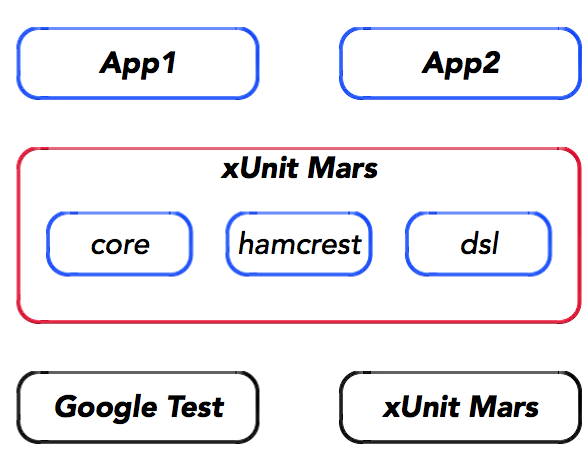
\includegraphics[width=0.4\textwidth]{figures/xunit/framework.png}
\caption{xUnit Mars: 系统架构}
 \label{fig:mars-framework}
\end{figure}

\end{content}

\section{破冰之旅}

\begin{content}

\subsection{环境准备}

创建一个项目并命名为\ascii{mars},然后在项目的顶层目录初始化一个空的\ascii{git}库。

\begin{leftbar}
 \begin{c++}[caption={\ttfamily{初始化git库}}] 
$ git init
 \end{c++}
\end{leftbar}  

\subsubsection{项目组织}

\ascii{xUnit Mars}项目的物理目录结构如下所示。

\begin{leftbar}
 \begin{c++}[caption={\ttfamily{项目组织}}]
mars
├── build
├── CMakeLists.txt
├── include
│   └── mars
├── src
│   ├── CMakeLists.txt
│   └── mars
└── test
    ├── CMakeLists.txt
    └── mars
 \end{c++}
\end{leftbar}

\subsubsection{构建工具}

\ascii{xUnit Mars}使用\ascii{CMake}构建工具,项目根目录下的主控\ascii{CMakeLists.txt}内容如下:

\begin{leftbar}
 \begin{c++}[caption={\ttfamily{CMakeLists.txt}}]
project(mars)                                                                                  
cmake_minimum_required(VERSION 2.8)

set(CMAKE_CXX_FLAGS "${CMAKE_CXX_FLAGS} -std=c++14")

include_directories("${CMAKE_CURRENT_SOURCE_DIR}/include")

add_subdirectory(src)
add_subdirectory(test)
 \end{c++}
\end{leftbar}

\ascii{src/CMakeLists.txt}完成\ascii{mars}库构建。

\begin{leftbar}
 \begin{c++}[caption={\ttfamily{src/CMakeLists.txt}}]
file(GLOB_RECURSE all_files *.cc)
add_library(mars STATIC ${all_files})
 \end{c++}
\end{leftbar}

\ascii{test/CMakeLists.txt}完成\ascii{mars-test}应用程序构建,它执行\ascii{xUnit Mars}项目的所有测试用例。

\begin{leftbar}
 \begin{c++}[caption={\ttfamily{test/CMakeLists.txt}}]
file(GLOB_RECURSE all_files *.cc)
add_executable(mars-test ${all_files})
target_link_libraries(mars-test mars gtest gtest_main pthread)
 \end{c++}
\end{leftbar}

项目组建完毕,提交代码。

\begin{leftbar}
 \begin{c++}[caption={\ttfamily{提交代码}}] 
$ git add .
$ git commit -m"setup project"
 \end{c++}
\end{leftbar}

\subsection{起航}

万事开头难,第一个用例跑起来并不容易。此处设计实现了一个简单的测试用例,用户通过扩展\ascii{xUnit Mars}框架中的\ascii{TestCase},新增新的测试用例。一般地,在面向对象设计中,扩展子类实现是遵循开放封闭原则的重要手段。

\begin{leftbar}
 \begin{c++}[caption={\ttfamily{test/mars/core/TestCaseSpec.cc}}]
#include <gtest/gtest.h>
#include "mars/core/TestCase.h"

namespace {
  struct SimpleTest : TestCase {
    bool wasRun = false;

  private:
    void run() override {
      wasRun = true;
    }
  };

  void run(TestCase& test) {
    test.run();
  }
}

TEST(SimpleTest, make_sure_test_case_can_run_normally) {
  SimpleTest test;
  run(test);

  ASSERT_TRUE(test.wasRun);
}
 \end{c++}
\end{leftbar}

\subsubsection{通过编译}

此处引入了多态技术,当\ascii{TestCase::run}启动运行时,将在运行时调用覆写的\ascii{SimpleTest::run},实现自定义测试用例的执行。

\begin{leftbar}
 \begin{c++}[caption={\ttfamily{include/mars/core/TestCase.h}}]
struct TestCase {
  virtual ~TestCase() {}
  virtual void run() = 0;
};
  \end{c++}
\end{leftbar}

\subsubsection{通过链接}

创建了一个空的\ascii{TestCase.cc}文件,仅为了\ascii{libmars.a}不为空,保证链接成功。

\begin{leftbar}
 \begin{c++}[caption={\ttfamily{src/mars/core/TestCase.cc}}]
#include "mars/core/TestCase.h"
 \end{c++}
\end{leftbar}

\begin{story}
  \begin{center}
    \inlinetitle{多屏编辑}
  \end{center}

\begin{content}

在\cpp{}编程实践中,需要在头文件和实现文件之间频繁切换。同时,在\ascii{TDD}编程实践中,也需要在测试文件与头文件/实现文件之间频繁切换。得益于现代\ascii{IDE}的丰富特性,推荐多屏显示相关源文件。例如,如\refig{multi-editor-eclipse}所示,使用\ascii{Eclipse CDT},三屏分别显示相关联的头文件、实现文件,及其测试用例文件。

\begin{figure}[H]
\centering
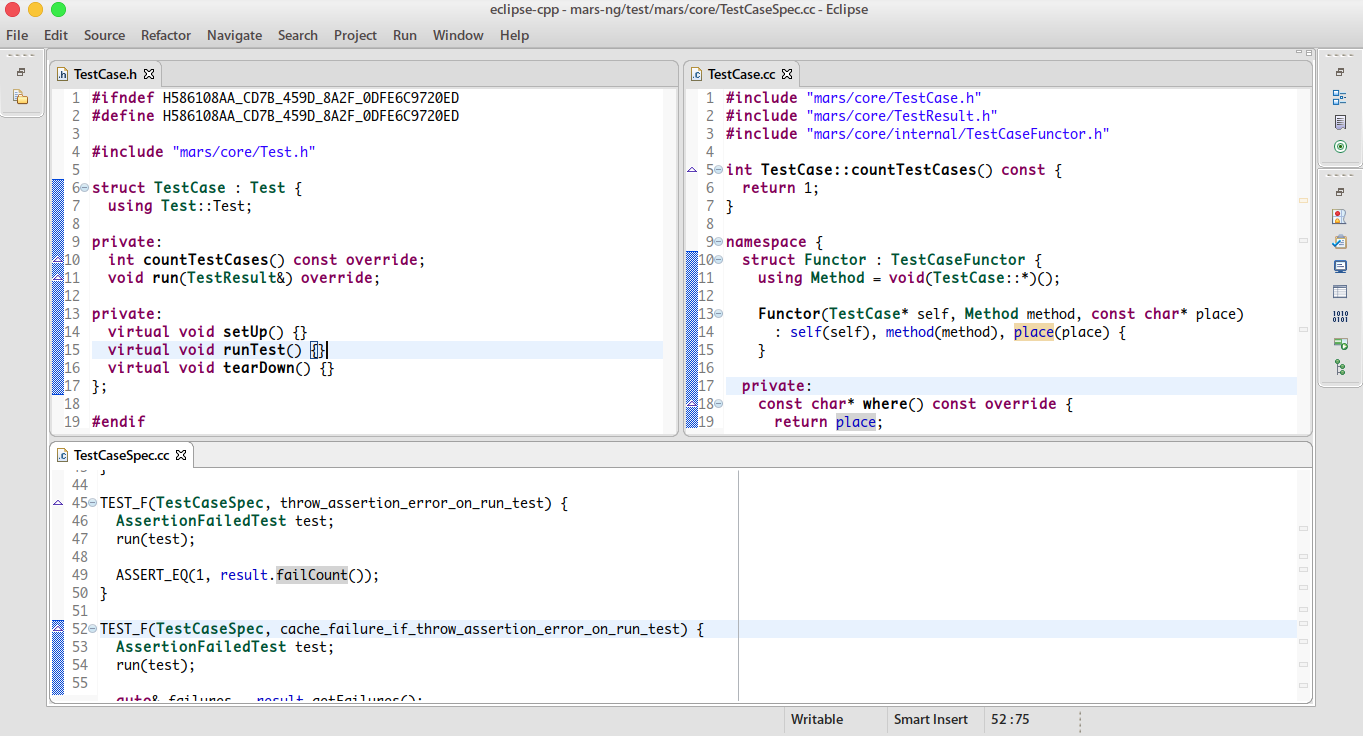
\includegraphics[width=1.0\textwidth]{figures/xunit/multi-editor-eclipse.png}
\caption{Eclipse CDT: 多屏显示}
 \label{fig:multi-editor-eclipse}
\end{figure}

因此,推荐购置高清,大屏的显示器,有效改善编程环境,从而提高工作效率。此外,推荐关闭其他无关的\ascii{Tab}页,只打开当前相关的源文件,最小化外部干扰;一则让\ascii{IDE}运行速度最佳,二则使用诸如\ascii{Ctrl + E}快捷键切换文件时,最小化文件列表长度。

强烈推荐使用快捷键的优秀实践,可以成倍地提高编程的效率。例如,使用\ascii{Eclipse CDT},可以使用快捷键\ascii{Ctrl + Tab},在头文件与实现文件间切换自如。

\end{content}

\end{story}

\subsubsection{通过测试}

在\ascii{build}临时目录中,使用\ascii{cmake}构建工程。

\begin{leftbar}
 \begin{c++}[caption={\ttfamily{构建工程}}]
$ mkdir -p build && cd build
$ cmake ..
$ make
 \end{c++}
\end{leftbar}

运行测试。

\begin{leftbar}
 \begin{c++}[caption={\ttfamily{运行测试}}]
$ test/mars-test
Running main() from gtest_main.cc
[==========] Running 1 test from 1 test case.
[----------] Global test environment set-up.
[----------] 1 test from SimpleTest
[ RUN      ] SimpleTest.make_sure_test_case_can_run_normally
[       OK ] SimpleTest.make_sure_test_case_can_run_normally (0 ms)
[----------] 1 test from SimpleTest (0 ms total)

[----------] Global test environment tear-down
[==========] 1 test from 1 test case ran. (0 ms total)
[  PASSED  ] 1 test.
 \end{c++}
\end{leftbar}

\subsubsection{提交代码}

每当通过测试后,立即提交代码到\ascii{Git}库。

\begin{leftbar}
 \begin{c++}[caption={\ttfamily{提交代码}}]
$ git add -A .
$ git commit -m"pass first test case"
 \end{c++}
\end{leftbar}

\begin{story}
  \begin{center}
    \inlinetitle{后悔药}
  \end{center}

\begin{content}

感谢\ascii{Linus}创造了\ascii{Linux}与\ascii{Git},让全世界的程序员享受编程的快乐。熟练运用\ascii{Git}工具,避免不经意的错误而丢失代码。

养成经常性提交代码至本地,是一种良好的编程习惯。在\ascii{TDD}实践的一个微循环中,当编译通过时,立即执行\ascii{git add};当链接通过时,立即执行\ascii{git add};当测试通过时,立即执行\ascii{git add};当完成重构的关键步骤时,也应该立即执行\ascii{git add};当重构完毕,设计达到合理状态,理解执行\ascii{git commit}。



\end{content}

\end{story}

\end{content}

\section{算法骨架}

\begin{content}

一般地,在执行测试前需要预置\ascii{setUp}实施测试环境的初始化工作,完成资源的准备。对既有的用例实施重构。

\subsection{前置}

\begin{leftbar}
 \begin{c++}[caption={\ttfamily{test/mars/core/TestCaseSpec.cc}}]
#include <gtest/gtest.h>
#include "mars/core/TestCase.h"

namespace {
  struct SimpleTest : TestCase {
    bool wasSetUp = false;
    bool wasRun = false;

  private:
    void setUp() override {
      wasSetUp = true;
    }

    void runTest() override {
      wasRun = true;
    }
  };
}

TEST(SimpleTest, make_sure_test_case_can_run_normally) {
  SimpleTest test;
  test.run();

  ASSERT_TRUE(test.wasSetUp);
  ASSERT_TRUE(test.wasRun);
}
 \end{c++}
\end{leftbar}

\subsubsection{通过编译}

重构\ascii{TestCase},仅公开\ascii{run}方法,并移除运行时多态的特性,它负责组织用例执行运行时的算法骨架。搬迁运行时多态行为至私有的两个虚函数,用户根据自己的场景定制\ascii{setUp}与\ascii{runTest},分别完成测试准备,及其测试执行。

\begin{leftbar}
 \begin{c++}[caption={\ttfamily{include/mars/core/TestCase.h}}]
struct TestCase {
  virtual ~TestCase() {}

  void run();

private:
  virtual void setUp() {}
  virtual void runTest() {}
};
  \end{c++}
\end{leftbar}

\subsubsection{通过测试}

实现\ascii{TestCase::run}的主体逻辑。

\begin{leftbar}
 \begin{c++}[caption={\ttfamily{src/mars/core/TestCase.cc}}]
#include "mars/core/TestCase.h"

void TestCase::run() {
  setUp();
  runTest();
}
 \end{c++}
\end{leftbar}

测试通过。

\subsection{后置}

同理,测试执行后使用\ascii{tearDown}完成现场清理,释放资源。用户通过定制私有的虚函数\ascii{tearDown}完成此功能。

\begin{leftbar}
 \begin{c++}[caption={\ttfamily{test/mars/core/TestCaseSpec.cc}}]
#include <gtest/gtest.h>
#include "mars/core/TestCase.h"

namespace {
  struct SimpleTest : TestCase {
    bool wasSetUp = false;
    bool wasRun = false;
    bool wasTearDown = false;

  private:
    void setUp() override {
      wasSetUp = true;
    }

    void runTest() override {
      wasRun = true;
    }

    void tearDown() override {
      wasTearDown = true;
    }
  };
}

TEST(SimpleTest, make_sure_test_case_can_run_normally) {
  SimpleTest test;
  test.run();

  ASSERT_TRUE(test.wasSetUp);
  ASSERT_TRUE(test.wasRun);
  ASSERT_TRUE(test.wasTearDown);  
}
 \end{c++}
\end{leftbar}

\subsubsection{通过编译}

当用例执行完成后,\ascii{TestCase::tearDown}负责清理现场。

\begin{leftbar}
 \begin{c++}[caption={\ttfamily{include/mars/core/TestCase.h}}]
struct TestCase {
  virtual ~TestCase() {}

  void run();

private:
  virtual void setUp() {}
  virtual void runTest() {}
  virtual void tearDown() {}
};
  \end{c++}
\end{leftbar}

\subsubsection{通过测试}

至此,完成了运行一个用例的主干逻辑,但缺乏异常处理机制,留待后续处理。

\begin{leftbar}
 \begin{c++}[caption={\ttfamily{src/mars/core/TestCase.cc}}]
#include "mars/core/TestCase.h"

void TestCase::run() {
  setUp();
  runTest();
  tearDown();
}
 \end{c++}
\end{leftbar}

\begin{figure}[H]
\centering
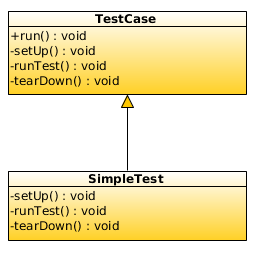
\includegraphics[width=0.4\textwidth]{figures/xunit/simple-test.png}
\caption{模板方法:定义算法骨架}
 \label{fig:simple-test}
\end{figure}

\end{content}

\section{隐式树}

\begin{content}

如果每个用例都需要手动地执行\ascii{run},显得极其笨拙。可以将一堆测试用例打包,用一个简单的\ascii{for}循环依次执行每个用例。

\subsection{测试套件}

为了确定每个\ascii{TestCase}都被执行,可以简单定制一个计数器\ascii{num},用例执行后,断言已运行用例的数目。

\begin{leftbar}
 \begin{c++}[caption={\ttfamily{test/mars/core/TestSuiteSpec.cc}}]
#include <gtest/gtest.h>
#include "mars/core/TestCase.h"
#include "mars/core/TestSuite.h"

namespace {
  int num = 0;

  struct FooTest : TestCase {
  private:
    void runTest() override {
      num++;
    }
  };
}

TEST(TestSuite, run_multi_test_cases_using_test_suite) {
  TestSuite suite;
  suite.add(new FooTest);
  suite.add(new FooTest);

  suite.run();

  ASSERT_EQ(2, num);
}
 \end{c++}
\end{leftbar}

\subsubsection{通过编译}

为了快速通过编译,创建\ascii{TestSuite}的头文件。

\begin{leftbar}
 \begin{c++}[caption={\ttfamily{include/mars/core/TestSuite.h}}]
#include <vector>

struct TestCase;

struct TestSuite {
  void add(TestCase* test);
  void run();

private:
  std::vector<TestCase*> tests;
};
 \end{c++}
\end{leftbar}

\subsubsection{通过测试}

为了通过测试,可以快速实现\ascii{TestSuite::run}的逻辑。

\begin{leftbar}
 \begin{c++}[caption={\ttfamily{src/mars/core/TestSuite.cc}}]
#include "mars/core/TestSuite.h"
#include "mars/core/TestCase.h"

void TestSuite::add(TestCase* test) {
  tests.push_back(test);
}

void TestSuite::run() {
  for (auto test : tests) {
    test->run();
  }
}
 \end{c++}
\end{leftbar}

\subsubsection{内存泄露}

\ascii{TestSuite}持有若干\ascii{TestCase}实例,引入析构函数释放动态创建并添加至\ascii{TestSuite}的所有\ascii{TestCase}实例。

\begin{leftbar}
 \begin{c++}[caption={\ttfamily{include/mars/core/TestSuite.h}}]
#include <vector>

struct TestCase;

struct TestSuite {
  ~TestSuite();

  void add(TestCase* test);
  void run();

private:
  std::vector<TestCase*> tests;
};
 \end{c++}
\end{leftbar}

实现析构函数,释放动态内存。

\begin{leftbar}
 \begin{c++}[caption={\ttfamily{src/mars/core/TestSuite.cc}}]
#include "mars/core/TestSuite.h"
#include "mars/core/TestCase.h"

void TestSuite::add(TestCase* test) {
  tests.push_back(test);
}

TestSuite::~TestSuite() {
  for (auto test : tests) {
    delete test;
  }
}

void TestSuite::run() {
  for (auto test : tests) {
    test->run();
  }
}
 \end{c++}
\end{leftbar}

\subsubsection{消除重复}

为了消除析构函数与\ascii{run}之间的重复代码,提取一个公共的\ascii{foreach}函数。注意,不要在头文件直接实现该模板函数,最小化编译时的依赖。

\begin{leftbar}
 \begin{c++}[caption={\ttfamily{include/mars/core/TestSuite.h}}]
#include <vector>

struct TestCase;

struct TestSuite {
  ~TestSuite();

  void add(TestCase* test);
  void run();

private:
  template <typename F>
  void foreach(F f) const;

private:
  std::vector<TestCase*> tests;
};
 \end{c++}
\end{leftbar}

因此,设计得到两个独立变化的方向。

\begin{enum}
  \eitem{\ascii{迭代算法:因存储结构变化而变化(目前实现为线性列表,不排除将来实现为map);}}
  \eitem{\ascii{处理算子:存在删除,计数,运行等操作。}}
\end{enum}

可以使用\ascii{Lambda}表达式定制各种算子,实现差异化配置,实现对迭代算法的高度复用。

\begin{leftbar}
 \begin{c++}[caption={\ttfamily{src/mars/core/TestSuite.cc}}]
#include "mars/core/TestSuite.h"
#include "mars/core/TestCase.h"

void TestSuite::add(TestCase* test) {
  tests.push_back(test);
}

template <typename F>
inline void TestSuite::foreach(F f) const {
  for (auto test : tests) {
    f(test);
  }
}

TestSuite::~TestSuite() {
  foreach([](auto test) {
    delete test;
  });
}

void TestSuite::run() {
  foreach([](auto test) {
    test->run();
  });
}
 \end{c++}
\end{leftbar}

\subsection{嵌套结构}

为了实现更好的可扩展性,\ascii{TestSuite}不仅能打包\ascii{TestCase}实例,也应该能够打包更小的\ascii{TestSuite}的子实例,实现隐式的树结构。


\begin{figure}[H]
\centering
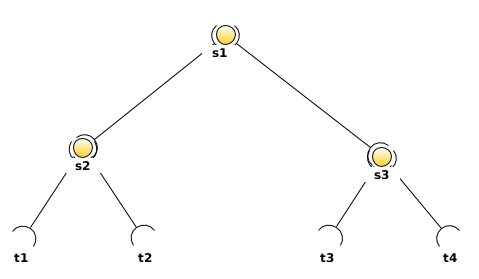
\includegraphics[width=0.8\textwidth]{figures/xunit/test-tree-example.png}
\caption{用例树:TestSuite(s1, s2, s3),TestCase(t1,t2,t3,t4)}
 \label{fig:simple-test}
\end{figure}

\subsubsection{测试依赖}

为了能够添加更多的用例,需要对计数器\ascii{num}实施初始化。当执行用例时,确保\ascii{num}被初始化为\ascii{0};否则测试用例之间存在数据脏写的错误依赖。另外,此处没有直接调用\ascii{TestSuite::run},而是使用更为抽象的\ascii{Test::run},测试装置将更加稳定。

在实现\ascii{TestSuiteSpec::run}时,显式地使用域限定符\ascii{::Test},避免与\ascii{testing::Test}产生二义性而导致编译失败。

\begin{leftbar}
 \begin{c++}[caption={\ttfamily{test/mars/core/TestSuiteSpec.cc}}]
#include <gtest/gtest.h>
#include "mars/core/TestCase.h"
#include "mars/core/TestSuite.h"

namespace {
  int num = 0;

  struct FooTest : TestCase {
  private:
    void runTest() override {
      num++;
    }
  };

  struct TestSuiteSpec : testing::Test {
  private:
    void SetUp() override {
      num = 0;  // IMPORTANT: reset counter.
    }

  protected:
    void run(::Test& test) {
      test.run();
    }
  };
}

TEST_F(TestSuiteSpec, package_multi_test_cases_into_test_suite) {
  TestSuite suite;
  suite.add(new FooTest);
  suite.add(new FooTest);

  run(suite);

  ASSERT_EQ(2, num);
}

TEST_F(TestSuiteSpec, package_sub_test_suite_into_outter_test_suite) {
  auto inner = new TestSuite;
  inner->add(new FooTest);

  TestSuite outter;
  outter.add(new FooTest);
  outter.add(inner);

  run(outter);

  ASSERT_EQ(2, num);
}
 \end{c++}
\end{leftbar}

此时,第二个测试用例编译失败。

\subsubsection{提取抽象}

通过提取\ascii{TestCase}与\ascii{TestSuite}的共同抽象\ascii{Test},从而使得用例的组织更加灵活。

\begin{leftbar}
 \begin{c++}[caption={\ttfamily{include/mars/core/Test.h}}]
struct Test {
  virtual ~Test() {}
  virtual void run() = 0;
};
 \end{c++}
\end{leftbar}

\subsubsection{重构TestCase}

重构\ascii{TestCase},所有显式声明的成员函数都是\ascii{private}。尤其关注被覆写的\ascii{TestCase::run},被显式地声明为\ascii{private},逼迫用户使用抽象接口\ascii{Test::run},而“面向接口编程”是一种良好的\ascii{OO}设计原则。

\begin{leftbar}
 \begin{c++}[caption={\ttfamily{include/mars/core/TestCase.h}}]
#include "mars/core/Test.h"

struct TestCase : Test {
private:
  void run() override;

private:
  virtual void setUp() {}
  virtual void runTest() {}
  virtual void tearDown() {}
};
 \end{c++}
\end{leftbar}

\subsubsection{重构TestSuite}

同理,\ascii{TestSuite}也应该被重构使用\ascii{Test}的抽象类型,而非使用\ascii{TestCase}的具体类型。

\begin{leftbar}
 \begin{c++}[caption={\ttfamily{include/mars/core/TestSuite.h}}]
#include <vector>
#include "mars/core/Test.h"

struct TestSuite : Test {
  ~TestSuite();
  void add(Test* test);

private:
  void run() override;

private:
  template <typename F>
  void foreach(F f) const;

private:
  std::vector<Test*> tests;
};
 \end{c++}
\end{leftbar}

同理,\ascii{TestSuite}的实现也应该使用\ascii{Test}的抽象类型。幸运的是,原来使用\ascii{auto}的自动类型推演,实现文件仅需要修改\ascii{TestSuite::add}函数签名便可以通过测试了。

\begin{leftbar}
 \begin{c++}[caption={\ttfamily{src/mars/core/TestSuite.cc}}]
#include "mars/core/TestSuite.h"

void TestSuite::add(Test* test) {
  tests.push_back(test);
}

template <typename F>
inline void TestSuite::foreach(F f) const {
  for (auto test : tests) {
    f(test);
  }
}

TestSuite::~TestSuite() {
  foreach([](auto test) {
    delete test;
  });
}

void TestSuite::run() {
  foreach([](auto test) {
    test->run();
  });
}
 \end{c++}
\end{leftbar}

通过\ascii{Test, TestCase, TestSuite}拼装组合,可以方便地构建复杂树形结构的用例图。

\begin{figure}[H]
\centering
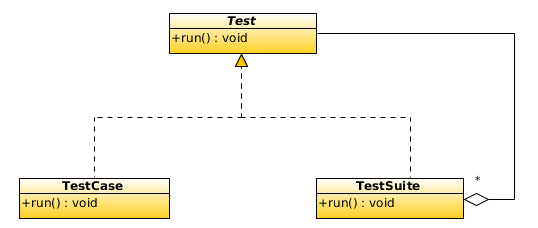
\includegraphics[width=0.8\textwidth]{figures/xunit/test-tree.png}
\caption{组合:构建隐式树}
 \label{fig:test-tree}
\end{figure}

\subsection{命名用例}

可以给每个\ascii{TestCase, TestSuite}命名,方便后期用例的定位与调试。

\begin{leftbar}
 \begin{c++}[caption={\ttfamily{test/mars/core/TestCaseSpec.cc}}]
#include <gtest/gtest.h>
#include "mars/core/TestCase.h"

namespace {
  void assertName(const Test& test, const char* expected) {
    ASSERT_EQ(std::string(expected), test.getName());
  }
}

TEST(NamedTestCase, named_test_case) {
  assertName(TestCase("test case1"), "test case1");
}
 \end{c++}
\end{leftbar}

\subsubsection{通过测试}

首先,增加抽象接口\ascii{Test::getName}。

\begin{leftbar}
 \begin{c++}[caption={\ttfamily{include/mars/core/Test.h}}]
#include <string>

struct Test {
  virtual ~Test() {}
  virtual const std::string& getName() const = 0;
  virtual void run() = 0;
};
 \end{c++}
\end{leftbar}

在\ascii{TestCase}中覆写\ascii{getName}成员函数。其中,为默认构造函数提供空字符串,保证既有的用例都能通过。

\begin{leftbar}
 \begin{c++}[caption={\ttfamily{include/mars/core/TestCase.h}}]
#include "mars/core/Test.h"

struct TestCase : Test {
  explicit TestCase(const std::string& = "");

private:
  const std::string& getName() const override;
  void run() override;

private:
  virtual void setUp() {}
  virtual void runTest() {}
  virtual void tearDown() {}

private:
  std::string name;
};
 \end{c++}
\end{leftbar}

在\ascii{TestCase.cc}中实现,也极为简单。

\begin{leftbar}
 \begin{c++}[caption={\ttfamily{include/mars/core/TestCase.h}}]
#include "mars/core/TestCase.h"

TestCase::TestCase(const std::string& name) : name(name) {
}

const std::string& TestCase::getName() const {
  return name;
}

// ...
 \end{c++}
\end{leftbar}

依葫芦画瓢,\ascii{TestSuite}的名字实现与\ascii{TestCase}雷同。

\begin{leftbar}
 \begin{c++}[caption={\ttfamily{include/mars/core/TestSuite.h}}]
#include <vector>
#include "mars/core/Test.h"

struct TestSuite : Test {
  explicit TestSuite(const std::string& = "");
  ~TestSuite();

  void add(Test* test);

private:
  const std::string& getName() const override;
  void run() override;

private:
  template <typename F>
  void foreach(F f) const;

private:
  std::string name;
  std::vector<Test*> tests;
};
 \end{c++}
\end{leftbar}

\begin{leftbar}
 \begin{c++}[caption={\ttfamily{include/mars/core/TestSuite.h}}]
#include "mars/core/TestSuite.h"

TestSuite::TestSuite(const std::string& name) : name(name) {
}

const std::string& TestSuite::getName() const {
  return name;
}

// ...
 \end{c++}
\end{leftbar}

至此,测试通过。

\subsubsection{消除重复}

但是,\ascii{TestCase}与\ascii{TestSuite}存在结构性重复设计,包括相同的构造函数,覆写\ascii{getName}成员函数,私有字段\ascii{name}。为了消除重复,重构将公共实现搬迁至父类。

搬迁至父类需要关注两点:

\begin{enum}
  \eitem{\ascii{Test}的构造函数被声明为\ascii{public},方便子类使用\ascii{using}语句直接复用构造函数。}
  \eitem{\ascii{getName}没有必要声明为虚函数,因为在\ascii{Test}内已经完全具备实现的条件;子类强制继承\ascii{getName}的实现,拒绝被覆写。}
\end{enum}

\begin{leftbar}
 \begin{c++}[caption={\ttfamily{include/mars/core/Test.h}}]
#include <string>

struct Test {
  explicit Test(const std::string& name = "");
  const std::string& getName() const;

  virtual ~Test() {}
  virtual void run() = 0;

private:
  std::string name;
};
 \end{c++}
\end{leftbar}

\ascii{Test::getName}实现异常简单。

\begin{leftbar}
 \begin{c++}[caption={\ttfamily{src/mars/core/Test.cc}}]
#include "mars/core/Test.h"

Test::Test(const std::string& name) : name(name) {
}

const std::string& Test::getName() const {
  return name;
}
 \end{c++}
\end{leftbar}

在\ascii{TestCase}中,直接使用\ascii{using}语句复用构造函数,删除既有的\ascii{TestCase::getName}实现,及其私有字段\ascii{std::string name}。

\begin{leftbar}
 \begin{c++}[caption={\ttfamily{include/mars/core/TestCase.h}}]
#include "mars/core/Test.h"

struct TestCase : Test {
  using Test::Test;

private:
  void run() override;

private:
  virtual void setUp() {}
  virtual void runTest() {}
  virtual void tearDown() {}
};
 \end{c++}
\end{leftbar}

同理,\ascii{TestSuite}中通过相同的手段实现代码复用。

\begin{leftbar}
 \begin{c++}[caption={\ttfamily{include/mars/core/TestSuite.h}}]
#include <vector>
#include "mars/core/Test.h"

struct TestSuite : Test {
  using Test::Test;

  ~TestSuite();

  void add(Test* test);

private:
  void run() override;

private:
  template <typename F>
  void foreach(F f) const;

private:
  std::vector<Test*> tests;
};
 \end{c++}
\end{leftbar}

遗憾的是,\ascii{Test}构造函数未能声明为\ascii{protected}。但是,即使\ascii{Test}的构造函数虽然被声明为\ascii{public},设计并未丢失编译时的安全检查。因为\ascii{Test::run}被声明为纯虚函数,在编译时保证用户无法直接创建\ascii{Test}实例。

\end{content}

\section{聚集参数}

\begin{content}

在之前的测试用例里,在匿名命名空间内引入计数器\ascii{num}。当某个用例被执行时,其\ascii{num++}。操作游离在对象之外的计数器是极为危险的,即使该计数器已经被限制在匿名命名空间内;因为,在其可见的作用域内都有可能被他人修改。

这是一种脆弱的设计,用户需要小心地维护计数器的初始化,也需要用户精细控制计数器累加的时机。一则容易引入不经意的错误,二则让计数器的操作散乱到各个子类覆写的\ascii{runTest}之中。

\subsection{引入TestResult}

为了消除这个不稳定的设计,这里引入\ascii{TestResult}的抽象,它专门负责计数器维护,及其测试结果收集等职责。重构测试用例,对外暴露\ascii{TestResult::runCount}的查询接口。

\begin{leftbar}
 \begin{c++}[caption={\ttfamily{test/mars/core/TestSuiteSpec.cc}}]
#include <gtest/gtest.h>
#include "mars/core/TestCase.h"
#include "mars/core/TestSuite.h"
#include "mars/core/TestResult.h"

namespace {
  struct TestSuiteSpec : testing::Test {
    void run(::Test& test) {
      test.run(result);
    }

  protected:
    TestResult result;
  };
}

TEST_F(TestSuiteSpec, run_multi_test_cases_using_test_suite) {
  TestSuite suite;
  suite.add(new TestCase);
  suite.add(new TestCase);

  run(suite);

  ASSERT_EQ(2, result.runCount());
}
 \end{c++}
\end{leftbar}

\subsubsection{实现TestResult}

\ascii{TestResult}维护了一个计数器,负责计数器初始化,累计操作数的职责。

\begin{leftbar}
 \begin{c++}[caption={\ttfamily{include/mars/core/TestResult.h}}]
struct TestResult {
  TestResult();

  void onRun();
  int runCount() const;

private:
  int numOfRuns;
};
 \end{c++}
\end{leftbar}

实现\ascii{TestResult}也较为简单。

\begin{leftbar}
 \begin{c++}[caption={\ttfamily{src/mars/core/TestResult.cc}}]
#include "mars/core/TestResult.h"

TestResult::TestResult() : numOfRuns(0) {
}

void TestResult::onRun() {
  numOfRuns++;
}

int TestResult::runCount() const {
  return numOfRuns;
}
 \end{c++}
\end{leftbar}

\subsubsection{重构TestCase}

当执行\ascii{TestCase::run}时,通知\ascii{TestResult}累加计数器。为了使得代码具有层次感,提取了\ascii{TestCase::runBare}的子函数,使得\ascii{TestCase::run}的主干更加清晰明了。

在头文件中,提取的\ascii{TestCase::runBare}的子函数声明为\ascii{private}。

\begin{leftbar}
 \begin{c++}[caption={\ttfamily{include/mars/core/TestCase.h}}]
#include "mars/core/Test.h"

struct TestCase : Test {
  using Test::Test;

private:
  void run(TestResult&) override;

private:
  virtual void setUp() {}
  virtual void runTest() {}
  virtual void tearDown() {}

private:
  void runBare();
};
 \end{c++}
\end{leftbar}

在实现文件中,搬迁主干逻辑至\ascii{TestCase::runBare}。

\begin{leftbar}
 \begin{c++}[caption={\ttfamily{src/mars/core/TestCase.cc}}]
#include "mars/core/TestCase.h"
#include "mars/core/TestResult.h"

void TestCase::runBare() {
  setUp();
  runTest();
  tearDown();
}

void TestCase::run(TestResult& result) {
  result.onRun();
  runBare();
}
 \end{c++}
\end{leftbar}

\subsubsection{重构TestSuite}

重构\ascii{TestSuite::run},每次迭代将\ascii{result}透传给\ascii{Test::run},实现多态调用。

\begin{leftbar}
 \begin{c++}[caption={\ttfamily{src/mars/core/TestSuite.cc}}]
#include "mars/core/TestSuite.h"

// ...

void TestSuite::run(TestResult& result) {
  foreach([&result](auto test) {
    test->run(result);
  });
}
 \end{c++}
\end{leftbar}

至此,测试通过。\ascii{TestResult}扮演了聚集参数的角色,它在运行时收集测试运行的结果。

\begin{figure}[H]
\centering
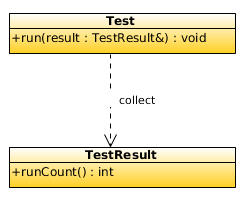
\includegraphics[width=0.4\textwidth]{figures/xunit/test-result.png}
\caption{聚集参数:收集测试结果}
 \label{fig:test-tree}
\end{figure}

\subsection{统计用例数目}

\ascii{TestResult::runCount}在运行时,通过监听接口统计测试用例的数目。事实上,也可以遍历用例树,直接统计测试用例的数目。构造一个失败的用例,观察如何统计测试用例数目。

\begin{leftbar}
 \begin{c++}[caption={\ttfamily{test/mars/core/TestSuiteSpec.cc}}]
#include <gtest/gtest.h>
#include "mars/core/TestCase.h"
#include "mars/core/TestSuite.h"
#include "mars/core/TestResult.h"

namespace {
  struct TestSuiteSpec : testing::Test {
    void run(::Test& test) {
      test.run(result);
    }

    int countTestCases(::Test& test) {
      return test.countTestCases();
    }

  protected:
    TestResult result;
  };
}

TEST_F(TestSuiteSpec, run_multi_test_cases_using_test_suite) {
  TestSuite suite;
  suite.add(new TestCase);
  suite.add(new TestCase);

  run(suite);

  ASSERT_EQ(2, countTestCases(suite));
}
 \end{c++}
\end{leftbar}

\subsubsection{通过编译}

增加\ascii{Test::countTestCases}纯虚接口。

\begin{leftbar}
 \begin{c++}[caption={\ttfamily{include/mars/core/Test.h}}]
#include <string>

struct TestResult;

struct Test {
  explicit Test(const std::string& name = "");
  const std::string& getName() const;

  virtual ~Test() {}
  virtual int countTestCases() const = 0;
  virtual void run(TestResult&) = 0;

private:
  std::string name;
};
 \end{c++}
\end{leftbar}

\ascii{TestCase::countTestCases}覆写行为直接返回\ascii{1}。

\begin{leftbar}
 \begin{c++}[caption={\ttfamily{src/mars/core/TestCase.cc}}]
int TestCase::countTestCases() const {
  return 1;
}
 \end{c++}
\end{leftbar}

\ascii{TestSuite::countTestCases}覆写行为完成\ascii{reduce}操作。

\begin{leftbar}
 \begin{c++}[caption={\ttfamily{src/mars/core/TestSuite.cc}}]
int TestSuite::countTestCases() const {
  auto num = 0;
  foreach([&num](auto test) {
    num += test->countTestCases();
  });
  return num;
}
 \end{c++}
\end{leftbar}

至此,测试通过。相对于\ascii{TestResult::runCount}通过聚集参数实现用例数目的统计,\ascii{TestResult::countTestCases}更加具有可扩展性;并且,\ascii{TestResult}与\ascii{TestCase}的耦合程度更小。

\end{content}

\section{异常处理}

\begin{content}

至此,框架不能处理任何异常逻辑。当用户调用\ascii{ASSERT\_EQ}失败时,抛出\ascii{AssertionError}异常,框架捕获该异常,标记该测试用例为\ascii{Failure};如果抛出其他异常,并被\ascii{mars}框架捕获,则标记该测试用例为\ascii{Error}。显式区分这两种异常类型,使得用户可以审查自己的测试用例,并修复失败的用例。

\subsection{断言失败}

当用例的断言失败,打印诸如如下详细信息,提示用户修复失败的用例。

\begin{leftbar}
 \begin{python}[caption={测试失败}]
/home/horance/code/cpp/mars/test/mars/core/TestCaseSpec.cc:33
expected value == 2, but got 0
 \end{python}
\end{leftbar}

接下来,构建失败的用例,在\ascii{runTest}时抛出异常\ascii{AssertionError},模拟断言失败的场景。

\begin{leftbar}
 \begin{c++}[caption={\ttfamily{test/mars/TestCaseSpec.cc}}]
#include <gtest/gtest.h>
#include "mars/core/TestCase.h"
#include "mars/except/AssertionError.h"

namespace {
  struct TestCaseSpec : testing::Test {
  protected:
    void run(::Test& test) {
      test.run(result);
    }

  protected:
    TestResult result;
  };

  struct AssertionFailedTest : TestCase {
    void runTest() override {
      throw AssertionError("test.cpp:57", "expected value == 2, but got 3");
    }
  };
}

TEST_F(TestCaseSpec, throw_assertion_error_on_run_test) {
  AssertionFailedTest test;
  run(test);

  ASSERT_EQ(1, result.failCount());
}
 \end{c++}
\end{leftbar}

\subsubsection{异常类}

为了通过编译,引入\ascii{AssertionError}的异常类。它携带了断言失败处的文件名与行号\ascii{(src)},及其用例断言失败的具体原因\ascii{(msg)}。

\begin{leftbar}
 \begin{c++}[caption={\ttfamily{include/mars/except/AssertionError.h}}]
#include <string>
#include <exception>

struct AssertionError : std::exception {
  AssertionError(const std::string& src, const std::string& msg);
  ~AssertionError() noexcept = default;

  const char* what() const noexcept;

private:
  std::string msg;
};
 \end{c++}
\end{leftbar}

\ascii{AssertionError}实现如下。

\begin{leftbar}
 \begin{c++}[caption={\ttfamily{src/mars/except/AssertionError.cc}}]
#include "mars/except/AssertionError.h"

AssertionError::AssertionError(const std::string& src,
  const std::string& msg) : msg(src + "\n" + msg) {
}

const char* AssertionError::what() const noexcept {
  return msg.c_str();
}
 \end{c++}
\end{leftbar}

\subsubsection{失败计数器}

\ascii{TestResult}新增名为\ascii{numOfFails}的计数器。

\begin{leftbar}
 \begin{c++}[caption={\ttfamily{include/mars/core/TestResult.h}}]
struct TestResult {
  TestResult();

  int failCount() const;
  void onFail();

private:
  int numOfFails;
};
 \end{c++}
\end{leftbar}

在实现文件中,实现失败计数器的初始化,累加,与查询逻辑。

\begin{leftbar}
 \begin{c++}[caption={\ttfamily{src/mars/core/TestResult.cc}}]
#include "mars/core/TestResult.h"

TestResult::TestResult() : numOfFails(0) {
}

int TestResult::failCount() const {
  return numOfFails;
}

void TestResult::onFail() {
  numOfFails++;
}
 \end{c++}
\end{leftbar}

\subsubsection{捕获异常}

当执行\ascii{TestCase::run}时,捕获异常并通过调用\ascii{TestResult::fail},累加计数器\ascii{numOfFails}。

\begin{leftbar}
 \begin{c++}[caption={\ttfamily{src/mars/core/TestCase.cc}}]
#include "mars/core/TestCase.h"
#include "mars/core/TestResult.h"
#include "mars/except/AssertionError.h"

void TestCase::run(TestResult& result) {
  setUp();

  try {
    runTest();
  } catch (const AssertionError&) {
    result.onFail();
  }

  tearDown();
}

// ...
 \end{c++}
\end{leftbar}

至此,测试通过。

\subsection{前置失败}

\ascii{TestCase}执行时,还未执行至\ascii{runTest}时,执行\ascii{setUp}可能就提前失败了。构建失败的用例,模拟前置失败的场景。

\begin{leftbar}
 \begin{c++}[caption={\ttfamily{test/mars/TestCaseSpec.cc}}]
namespace {
  struct AssertionFailedOnSetUpTest : TestCase {
    bool wasRun = false;

  private:
    void setUp() override {
      throw AssertionError("test.cpp:57", "expected value == 2, but got 3");
    }

    void runTest() override {
      wasRun = true;
    }
  };
}

TEST_F(TestCaseSpec, throw_assertion_error_on_setup) {
  AssertionFailedOnSetUpTest test;
  run(test);

  ASSERT_EQ(1, result.failCount());
  ASSERT_FALSE(test.wasRun);
}
 \end{c++}
\end{leftbar}

\subsubsection{捕获异常}

为了通过测试,当执行\ascii{TestCase::setUp}时,捕获异常并通知\ascii{TestResult},然后立即终止用例的执行;毕竟环境没准备好,强制执行用例毫无意义。

\begin{leftbar}
 \begin{c++}[caption={\ttfamily{src/mars/core/TestCase.cc}}]
#include "mars/core/TestCase.h"
#include "mars/core/TestResult.h"
#include "mars/except/AssertionError.h"

void TestCase::run(TestResult& result) {
  bool succ = false;
  try {
    setUp();
    succ = true;
  } catch (const AssertionError&) {
    result.onFail();
  }

  if (succ) {
    try {
      runTest();
    } catch (const AssertionError&) {
      result.onFail();
    }
  }

  tearDown();
}
 \end{c++}
\end{leftbar}

至此,测试通过。

\subsection{后置失败}

\ascii{TestCase::runBare}执行时,执行完\ascii{setUp, runTest}成功之后,接着执行\ascii{tearDown}时失败。构建失败的用例,模拟后置失败的场景。

\begin{leftbar}
 \begin{c++}[caption={\ttfamily{test/mars/TestCaseSpec.cc}}]
namespace {
  struct AssertionFailedOnTearDownTest : TestCase {
    void tearDown() override {
      throw AssertionError("test.cpp:57", "expected value == 2, but got 3");
    }
  };
}

TEST_F(TestCaseSpec, throw_assertion_error_on_tear_down) {
  AssertionFailedOnTearDownTest test;
  run(test);

  ASSERT_EQ(1, result.failCount());
}
 \end{c++}
\end{leftbar}

\subsubsection{捕获异常}

当执行\ascii{TestCase::tearDown}时,捕获异常并通知\ascii{TestResult}。但是,无论\ascii{setUp, runTest}成败与否,\ascii{tearDown}都要强制执行,保证资源的安全释放。

\begin{leftbar}
 \begin{c++}[caption={\ttfamily{src/mars/core/TestCase.cc}}]
#include "mars/core/TestCase.h"
#include "mars/core/TestResult.h"
#include "mars/except/AssertionError.h"

void TestCase::run(TestResult& result) {
  bool succ = false;
  try {
    setUp();
    succ = true;
  } catch (const AssertionError&) {
    result.onFail();
  }

  if (succ) {
    try {
      runTest();
    } catch (const AssertionError&) {
      result.onFail();
    }
  }

  try {
    tearDown();
  } catch (const AssertionError&) {
    result.onFail();
  }
}
 \end{c++}
\end{leftbar}

至此,测试通过。

\subsection{失败与错误}

当抛出\ascii{AssertionError},称之为\ascii{Failure};当抛出其他异常,称之为\ascii{Error}。构建失败的用例,模拟其他异常抛出的场景。

\begin{leftbar}
 \begin{c++}[caption={\ttfamily{test/mars/TestCaseSpec.cc}}]
namespace {
  struct StdExceptionTest : TestCase {
    void runTest() override {
      throw std::exception();
    }
  };
}

TEST_F(TestCaseSpec, throw_std_exception_on_run_test) {
  StdExceptionTest test;
  run(test);

  ASSERT_EQ(0, result.failCount());
  ASSERT_EQ(1, result.errorCount());
}
 \end{c++}
\end{leftbar}

\subsubsection{错误计数器}

增加查询函数\ascii{TestResult::errorCount}查询函数,错误监听接口\ascii{TestResult::onError},及其相应的错误计数器\ascii{numOfErrors}。

\begin{leftbar}
 \begin{c++}[caption={\ttfamily{include/mars/core/TestResult.h}}]
struct TestResult {
  TestResult();

  int failCount() const;
  int errorCount() const;

  void onFail();
  void onError();

private:
  int numOfFails;
  int numOfErrors;
};
 \end{c++}
\end{leftbar}

在实现文件中,依葫芦画瓢,实现\ascii{TestResult::errorCount, TestResult::onError}。

\begin{leftbar}
 \begin{c++}[caption={\ttfamily{src/mars/core/TestResult.cc}}]
#include "mars/core/TestResult.h"

TestResult::TestResult()
  : numOfFails(0), numOfErrors(0) {
}

int TestResult::failCount() const {
  return numOfFails;
}

int TestResult::errorCount() const {
  return numOfErrors;
}

void TestResult::onFail() {
  numOfFails++;
}

void TestResult::onError() {
  numOfErrors++;
}
 \end{c++}
\end{leftbar}

\subsubsection{捕获异常}

当执行\ascii{TestCase::runTest}时,捕获\ascii{std::exception}异常,并通知\ascii{TestResult::error}累加计数器。

\begin{leftbar}
 \begin{c++}[caption={\ttfamily{src/mars/core/TestCase.cc}}]
#include "mars/core/TestCase.h"
#include "mars/core/TestResult.h"
#include "mars/except/AssertionError.h"

void TestCase::run(TestResult& result) {
  bool succ = false;
  try {
    setUp();
    succ = true;
  } catch (const AssertionError&) {
    result.onFail();
  }

  if (succ) {
    try {
      runTest();
    } catch (const AssertionError&) {
      result.onFail();
    } catch (const std::exception&) {
      result.onError();
    }
  }

  try {
    tearDown();
  } catch (const AssertionError&) {
    result.onFail();
  }
}
 \end{c++}
\end{leftbar}

\subsection{未知错误}

当抛出其他未知的异常,测试框架需要捕获,并标记为\ascii{Error},提示用户被测系统存在严重的漏洞。

\begin{leftbar}
 \begin{c++}[caption={\ttfamily{test/mars/TestCaseSpec.cc}}]
namespace {
  struct UnknownException {};

  struct UnknownExceptionTest : TestCase {
    void runTest() override {
      throw UnknownException();
    }
  };
}

TEST_F(TestCaseSpec, throw_unknown_exception_on_run_test) {
  UnknownExceptionTest test;
  run(test);

  ASSERT_EQ(0, result.failCount());
  ASSERT_EQ(1, result.errorCount());
}
 \end{c++}
\end{leftbar}

\subsubsection{捕获异常}

当执行\ascii{TestCase::runTest}时,捕获未知的异常,并通知\ascii{TestResult::error}累加计数器。

\begin{leftbar}
 \begin{c++}[caption={\ttfamily{src/mars/core/TestCase.cc}}]
#include "mars/core/TestCase.h"
#include "mars/core/TestResult.h"
#include "mars/except/AssertionError.h"

void TestCase::run(TestResult& result) {
  bool succ = false;
  try {
    setUp();
    succ = true;
  } catch (const AssertionError&) {
    result.onFail();
  }

  if (succ) {
    try {
      runTest();
    } catch (const AssertionError&) {
      result.onFail();
    } catch (const std::exception&) {
      result.onError();
    } catch (...) {
      result.onError();
    }    
  }

  try {
    tearDown();
  } catch (const AssertionError&) {
    result.onFail();
  }
}
 \end{c++}
\end{leftbar}

测试通过。

\subsection{完备的异常处理}

依次构建测试用例,小步快走,驱动出完备的异常处理逻辑。

\begin{leftbar}
 \begin{c++}[caption={\ttfamily{src/mars/core/TestCase.cc}}]
#include "mars/core/TestCase.h"
#include "mars/core/TestResult.h"
#include "mars/except/AssertionError.h"

void TestCase::run(TestResult& result) {
  bool succ = false;
  try {
    setUp();
    succ = true;
  } catch (const AssertionError&) {
    result.onFail();
  } catch (const std::exception&) {
    result.onError();
  } catch (...) {
    result.onError();
  }

  if (succ) {
    try {
      runTest();
    } catch (const AssertionError&) {
      result.onFail();
    } catch (const std::exception&) {
      result.onError();
    } catch (...) {
      result.onError();
    }
  }

  try {
    tearDown();
  } catch (const AssertionError&) {
    result.onFail();
  } catch (const std::exception&) {
    result.onError();
  } catch (...) {
    result.onError();
  }
}

// ...
 \end{c++}
\end{leftbar}

\ascii{TestCase::run}实现不仅存在重复逻辑,而且异常臃肿,异常丑陋。此时不重构,更待何时。

\subsubsection{消除重复}

观察\ascii{TestCase::setUp, TestCase::runTest, TestCase::tearDown}的共性,它们拥有相同的函数签名,可以使用指向成员函数的指针挖掘它们的共性。

\begin{leftbar}
 \begin{c++}
using Method = void(TestCase::*)();
 \end{c++}
\end{leftbar}

提取公共函数\ascii{TestCase::protect},它返回\ascii{bool}类型。首先,在头文件中声明私有函数\ascii{TestCase::protect}。

\begin{leftbar}
 \begin{c++}[caption={\ttfamily{include/mars/core/TestCase.h}}]
#include "mars/core/Test.h"

struct TestCase : Test {
  using Test::Test;

private:
  int countTestCases() const override;
  void run(TestResult&) override;

private:
  virtual void setUp() {}
  virtual void runTest() {}
  virtual void tearDown() {}

private:
  using Method = void(TestCase::*)();
  bool protect(TestResult& result, Method method);
};
 \end{c++}
\end{leftbar}

在实现文件中,实现异常处理逻辑的代码复用。

\begin{leftbar}
 \begin{c++}[caption={\ttfamily{src/mars/core/TestCase.cc}}]
#include "mars/core/TestCase.h"
#include "mars/core/TestResult.h"
#include "mars/except/AssertionError.h"

bool TestCase::protect(TestResult& result, Method method) {
  bool succ = false;
  try {
    (this->*method)();
    succ = true;
  } catch (const AssertionError&) {
    result.onFail();
  } catch (const std::exception&) {
    result.onError();
  } catch (...) {
    result.onError();
  }
  return succ;
}

void TestCase::run(TestResult& result) {
  if (protect(result, &TestCase::setUp)) {
    protect(result, &TestCase::runTest);
  }
  protect(result, &TestCase::tearDown);
}

int TestCase::countTestCases() const {
  return 1;
}
 \end{c++}
\end{leftbar}

\end{content}

\section{解耦合}

\begin{content}

分析\ascii{TestCase}实现,\ascii{TestCase::setUp, TestCase::runTest, TestCase::tearDown}宿主于\ascii{TestCase},而异常处理逻辑主要宿主于\ascii{TestResult}。

根据迪米特法则,这段异常处理的逻辑应搬迁至\ascii{TestResult}。当捕获异常后,直接更新到自己的私有数据域,使得\ascii{TestResult::onRun, TestResult::onFail, TestResult::onError}等监听接口完全私有化。

但是,\ascii{TestResult}如何调用到\ascii{TestCase::setUp, TestCase::runTest, TestCase::tearDown}成员函数呢?此时似乎陷入窘境,毕竟\ascii{TestCase}与\ascii{TestResult}之间的耦合太过紧密,拆分显得不是那么容易。

解除\ascii{TestCase}与\ascii{TestResult}之间的耦合迫在眉睫。

\subsection{关键抽象: TestCaseFunctor}

为了彻底解开\ascii{TestCase::protect}对\ascii{TestCase}的依赖,引入关键抽象\ascii{TestCaseFunctor},相对\ascii{TestCase::Method}的简单抽象,它更加稳定,更加具有可扩展性(可以携带更多元数据,例如增加\ascii{getTestName}接口)。

\begin{leftbar}
 \begin{c++}[caption={\ttfamily{include/mars/core/internal/TestCaseFunctor.h}}]
#include <string>

struct TestCaseFunctor {
  virtual ~TestCaseFunctor() {}
  virtual bool operator()() const = 0;
};
 \end{c++}
\end{leftbar}

\subsubsection{实现TestCaseFunctor}

在\ascii{TestCase.h}的文件中,修改\ascii{TestCase::protect}的声明,让其依赖于更稳定的抽象\ascii{TestCaseFunctor},而非简单抽象\ascii{TestCase::Method},因为\ascii{TestCaseFunctor}不包含\ascii{TestCase}的任何信息。

\begin{leftbar}
 \begin{c++}[caption={\ttfamily{include/mars/core/TestCase.h}}]
#include "mars/core/Test.h"

struct TestCaseFunctor;

struct TestCase : Test {
  using Test::Test;

private:
  int countTestCases() const override;
  void run(TestResult&) override;

private:
  virtual void setUp() {}
  virtual void runTest() {}
  virtual void tearDown() {}

private:
  bool protect(TestResult&, const TestCaseFunctor&);
};
 \end{c++}
\end{leftbar}

在\ascii{TestCase.cc}实现文件中,在匿名命名空间内定义实现\ascii{Functor},它是\ascii{TestCaseFunctor}背后运行的真正实现,它包装实现了原来\ascii{TestCase::Method}的间接调用。

\begin{leftbar}
 \begin{c++}[caption={\ttfamily{src/mars/core/TestCase.cc}}]
#include "mars/core/TestCase.h"
#include "mars/core/TestResult.h"
#include "mars/core/internal/TestCaseFunctor.h"
#include "mars/except/AssertionError.h"

namespace {
  struct Functor : TestCaseFunctor {
    using Method = void(TestCase::*)();

    Functor(TestCase* self, Method method)
      : self(self), method(method) {
    }

  private:
    bool operator()() const override {
      (self->*method)();
      return true;
    }

  private:
    TestCase* self;
    Method method;
  };
}

bool TestCase::protect(TestResult& result, const TestCaseFunctor& f) {
  try {
    return f();
  } catch (const AssertionError&) {
    result.onFail();
  } catch (const std::exception&) {
    result.onError();
  } catch (...) {
    result.onError();
  }
  return false;
}

void TestCase::run(TestResult& result) {
  if (protect(result, Functor(this, &TestCase::setUp))) {
    protect(result, Functor(this, &TestCase::runTest));
  }
  protect(result, Functor(this, &TestCase::tearDown));
}
 \end{c++}
\end{leftbar}

\subsection{搬迁异常逻辑}

运用迪米特法则,将异常处理的逻辑从\ascii{TestCase::protect}搬迁至\ascii{TestResult::protect}。因为\ascii{TestResult::protect}依赖与\ascii{TestCaseFunctor}的抽象类型,而非具体的\ascii{TestCase},实现了\ascii{TestResult}对\ascii{TestCase}的解耦。在头文件中,公开\ascii{TestResult::protect},而私有\ascii{onFail, onError}。

\begin{leftbar}
 \begin{c++}[caption={\ttfamily{include/mars/core/TestResult.h}}]
struct TestCaseFunctor;

struct TestResult {
  TestResult();

  int failCount() const;
  int errorCount() const;

  bool protect(const TestCaseFunctor&);

private:
  void onFail();
  void onError();

private:
  int numOfFails;
  int numOfErrors;
};
 \end{c++}
\end{leftbar}

在实现文件中,搬迁异常处理逻辑至此处。

\begin{leftbar}
 \begin{c++}[caption={\ttfamily{src/mars/core/TestResult.cc}}]
#include "mars/core/TestResult.h"
#include "mars/core/internal/TestCaseFunctor.h"
#include "mars/except/AssertionError.h"

bool TestResult::protect(const TestCaseFunctor& f) {
  try {
    return f();
  } catch (const AssertionError&) {
    onFail();
  } catch (const std::exception&) {
    onError();
  } catch (...) {
    onError();
  }
  return false;
}
 \end{c++}
\end{leftbar}

\subsubsection{重构TestCase}

重构\ascii{TestCase},使其调用\ascii{TestResult::protect}完成异常处理的逻辑。测试通过后,删除既有的\ascii{TestCase::protect}。

\begin{leftbar}
 \begin{c++}[caption={\ttfamily{src/mars/core/TestCase.cc}}]
#include "mars/core/TestCase.h"
#include "mars/core/TestResult.h"
#include "mars/core/internal/TestCaseFunctor.h"

namespace {
  struct Functor : TestCaseFunctor {
    using Method = void(TestCase::*)();

    Functor(TestCase* self, Method method)
      : self(self), method(method) {
    }

  private:
    bool operator()() const override {
      (self->*method)();
      return true;
    }

  private:
    TestCase* self;
    Method method;
  };
}

void TestCase::run(TestResult& result) {
  if (result.protect(Functor(this, &TestCase::setUp))) {
    result.protect(Functor(this, &TestCase::runTest));
  }
  result.protect(Functor(this, &TestCase::tearDown));
}
 \end{c++}
\end{leftbar}

\subsubsection{改善表达力}

可以定义一个宏,改善\ascii{TestCase::run}对\ascii{TestResult::protect}调用的表达力。不忘初心,\ascii{TestCase::run}算法主干回归至最开始的简单逻辑。

\begin{leftbar}
 \begin{c++}[caption={\ttfamily{src/mars/core/TestCase.cc}}]
#define PROTECT(method) \
    result.protect(Functor(this, &TestCase::method))

void TestCase::run(TestResult& result) {
  if (PROTECT(setUp)) {
    PROTECT(runTest);
  }
  PROTECT(tearDown);
}
 \end{c++}
\end{leftbar}

\end{content}

\section{异常信息}

\begin{content}

当用例失败后,用户期望终端打印如下信息,方便用户快速修复失败的用例。

\begin{leftbar}
 \begin{c++}[caption={\ttfamily{include/mars/except/TestFailure.h}}]
assertion fail in the runTest
/home/horance/code/cpp/cut/test/hamcrest/core/ComparatorTest.cpp:12
Expected: a value eq <254: int>
     but: <255: int> eq <254: int> got false
 \end{c++}
\end{leftbar}

异常信息包括如下几个重要逻辑信息:

\begin{enum}
  \eitem{\ascii{Why}: 指明用例失败的原因}
    \begin{enum}
      \eitem{\ascii{assertion fail}: 断言失败}
      \eitem{\ascii{uncaught std::exception}: 被测系统抛出\ascii{std::exception}或子异常}
      \eitem{\ascii{uncaught unknown exception}: 被测系统抛出其他未知异常}
    \end{enum}
  \eitem{\ascii{Where}: 异常抛出的地点}
    \begin{enum}
      \eitem{\ascii{in the setUp}}
      \eitem{\ascii{in the runTest}}
      \eitem{\ascii{in the tearDown}}
    \end{enum}
  \eitem{\ascii{What}: 异常携带的详细信息}
    \begin{enum}
      \eitem{\ascii{源文件}}
      \eitem{\ascii{行号}}
      \eitem{\ascii{异常详细信息}: \ascii{what}成员函数返回值}
    \end{enum}
\end{enum}

\subsection{断言失败}

重构既有的测试用例,当\ascii{runTest}因断言失败而抛出\ascii{AssertionError},\ascii{TestResult}缓存异常信息。

\begin{leftbar}
 \begin{c++}[caption={\ttfamily{test/mars/core/TestCaseSpec.cc}}]
namespace {
  struct AssertionFailedTest : TestCase {
    const char* expectMsg() const {
      return "assertion fail in the runTest\n"
              "TestCaseSpec.cpp:57\n"
              "expected value == 2, but got 3";
    }

  private:
    void runTest() override {
      throw AssertionError("TestCaseSpec.cpp:57", "expected value == 2, but got 3");
    }
  };
}

TEST_F(TestCaseSpec, throw_assertion_error_on_run_test) {
  AssertionFailedTest test;
  run(test);

  ASSERT_EQ(1, result.failCount());
  ASSERT_FALSE(result.getFailures().empty());
  ASSERT_EQ(test.expectMsg(), result.getFailures().front());
}
 \end{c++}
\end{leftbar}

\subsubsection{缓存异常信息}

\ascii{TestResult}建立相应的数据结构,缓存异常信息;同时,对外提供\ascii{getFailures}的查询接口,供外部用户获取异常信息。

\begin{leftbar}
 \begin{c++}[caption={\ttfamily{include/mars/core/TestResult.h}}]
#include <vector>
#include <string>

struct TestCaseFunctor;

struct TestResult {
  TestResult();

  int failCount() const;
  int errorCount() const;

  bool protect(const TestCaseFunctor&);

  const std::vector<std::string>& getFailures() const;

private:
  void onFail(std::string&& msg);
  void onError();

private:
  int numOfFails;
  int numOfErrors;

  std::vector<std::string> failures;
};
 \end{c++}
\end{leftbar}

当异常被捕获后,通过\ascii{onFail}监听接口添加至缓存。

\begin{leftbar}
 \begin{c++}[caption={\ttfamily{src/mars/core/TestResult.cc}}]
#include "mars/core/TestResult.h"
#include "mars/except/AssertionError.h"

// ...

const std::vector<std::string>& TestResult::getFailures() const {
  return failures;
}

bool TestResult::protect(const TestCaseFunctor& f) {
  try {
    return f();
  } catch (const AssertionError& e) {
    onFail(std::string("assertion fail") + " " + f.where() + "\n" + e.what());
  } catch (const std::exception& e) {
    onError();
  } catch (...) {
    onError();
  }
  return false;
}

void TestResult::onFail(std::string&& msg) {
  failures.emplace_back(std::move(msg));
  numOfFails++;
}
 \end{c++}
\end{leftbar}

\subsubsection{获取异常位置}

得益于\ascii{TestCaseFunctor}的可扩展性,可以扩展增加查询接口,可以方便携带额外的元数据。

\begin{leftbar}
 \begin{c++}[caption={\ttfamily{src/mars/core/TestResult.cc}}]
struct TestCaseFunctor {
  virtual ~TestCaseFunctor() {}
  virtual const char* where() const = 0;
  virtual bool operator()() const = 0;
};
 \end{c++}
\end{leftbar}

在\ascii{TestCase::run}实现中,通过修改\ascii{PROTECT}宏定义,并在匿名命名空间覆写\ascii{where}成员函数,报告异常发生的位置信息。

\begin{leftbar}
 \begin{c++}[caption={\ttfamily{src/mars/core/TestResult.cc}}]
namespace {
  struct Functor : TestCaseFunctor {
    using Method = void(TestCase::*)();

    Functor(TestCase* self, Method method, const char* place)
      : self(self), method(method), place(place) {
    }

  private:
    const char* where() const override {
      return place;
    }

    bool operator()() const override {
      (self->*method)();
      return true;
    }

  private:
    TestCase* self;
    Method method;
    const char* place;
  };
}

#define PROTECT(method) \
    result.protect(Functor(this, &TestCase::method, "in the "#method))

void TestCase::run(TestResult& result) {
  if (PROTECT(setUp)) {
    PROTECT(runTest);
  }
  PROTECT(tearDown);
}
 \end{c++}
\end{leftbar}

\subsection{错误: 抛出std::exception}

模拟在\ascii{runTest}抛出错误,并断言异常信息。

\begin{leftbar}
 \begin{c++}[caption={\ttfamily{test/mars/core/TestCaseSpec.cc}}]
namespace {
  struct StdExceptionTest : TestCase {
    const char* expectMsg() const {
      return "uncaught std::exception in the runTest\n"
             "std::exception";
    }

  private:
    void runTest() override {
      throw std::exception();
    }
  };
}

TEST_F(TestCaseSpec, throw_std_exception_on_run_test) {
  StdExceptionTest test;
  run(test);

  ASSERT_EQ(0, result.failCount());
  ASSERT_EQ(1, result.errorCount());

  auto& errors = result.getErrors();
  ASSERT_FALSE(errors.empty());
  ASSERT_EQ(test.expectMsg(), errors.front());
}
 \end{c++}
\end{leftbar}

\subsubsection{缓存错误信息}

依葫芦画瓢,\ascii{TestResult}增加查询接口\ascii{getErrors},重构监听异常接口\ascii{onError}。

\begin{leftbar}
 \begin{c++}[caption={\ttfamily{include/mars/core/TestResult.h}}]
#include <vector>
#include <string>

struct TestCaseFunctor;

struct TestResult {
  TestResult();

  int failCount() const;
  int errorCount() const;

  bool protect(const TestCaseFunctor&);

  const std::vector<std::string>& getFailures() const;
  const std::vector<std::string>& getErrors() const;

private:
  void onFail(std::string&& msg);
  void onError(std::string&& msg);

private:
  int numOfFails;
  int numOfErrors;

  std::vector<std::string> failures;
  std::vector<std::string> errors;
};
 \end{c++}
\end{leftbar}

在实现文件中,与之前的实现雷同。

\begin{leftbar}
 \begin{c++}[caption={\ttfamily{src/mars/core/TestResult.cc}}]
#include "mars/core/TestResult.h"
#include "mars/core/internal/TestCaseFunctor.h"
#include "mars/except/AssertionError.h"

// ...

const std::vector<std::string>& TestResult::getFailures() const {
  return failures;
}

const std::vector<std::string>& TestResult::getErrors() const {
  return errors;
}

bool TestResult::protect(const TestCaseFunctor& f) {
  try {
    return f();
  } catch (const AssertionError& e) {
    onFail(std::string("assertion fail") + " " + f.where() + "\n" + e.what());
  } catch (const std::exception& e) {
    onError(std::string("uncaught std::exception") + " " + f.where() + "\n" + e.what());
  } catch (...) {
    onError("");
  }
  return false;
}

void TestResult::onFail(std::string&& msg) {
  failures.emplace_back(std::move(msg));
  numOfFails++;
}

void TestResult::onError(std::string&& msg) {
  errors.emplace_back(std::move(msg));
  numOfErrors++;
}
 \end{c++}
\end{leftbar}

\subsection{未知错误}

遵循上述微步的循环,驱动实现未知错误的缓存特性。最终,\ascii{TestResult::protect}的异常处理逻辑如下所示。

\begin{leftbar}
 \begin{c++}[caption={\ttfamily{src/mars/core/TestResult.cc}}]
#include "mars/core/TestResult.h"
#include "mars/core/internal/TestCaseFunctor.h"
#include "mars/except/AssertionError.h"

// ...

const std::vector<std::string>& TestResult::getFailures() const {
  return failures;
}

const std::vector<std::string>& TestResult::getErrors() const {
  return errors;
}

bool TestResult::protect(const TestCaseFunctor& f) {
  try {
    return f();
  } catch (const AssertionError& e) {
    onFail(std::string("assertion fail") + " " + f.where() + "\n" + e.what());
  } catch (const std::exception& e) {
    onError(std::string("uncaught std::exception") + " " + f.where() + "\n" + e.what());
  } catch (...) {
    onError(std::string("uncaught unknown exception") + " " + f.where() + "\n" + "");
  }
  return false;
}

void TestResult::onFail(std::string&& msg) {
  failures.emplace_back(std::move(msg));
  numOfFails++;
}

void TestResult::onError(std::string&& msg) {
  errors.emplace_back(std::move(msg));
  numOfErrors++;
}
 \end{c++}
\end{leftbar}

\subsection{引入值对象}

使用字符串表示异常信息是一种脆弱的设计,可以将其重构为值对象,从而得到更稳定的设计。首先,重构既有的测试用例,使其失败。

\begin{leftbar}
 \begin{c++}[caption={\ttfamily{test/mars/core/TestCaseSpec.cc}}]
namespace {
  struct AssertionFailedTest : TestCase {
    const char* expectMsg() const {
      return "assertion fail in the runTest\n"
             "test.cpp:57\n"
             "expected value == 2, but got 3";
    }

  private:
    void runTest() override {
      throw AssertionError("test.cpp:57", "expected value == 2, but got 3");
    }
  };
}

TEST_F(TestCaseSpec, cache_failure_if_throw_assertion_error_on_run_test) {
  AssertionFailedTest test;
  run(test);

  auto& failures = result.getFailures();
  ASSERT_FALSE(failures.empty());

  auto failure = failures.front();
  ASSERT_TRUE(failure->isFailure());
  ASSERT_EQ(test.expectMsg(), failure->getExceptionMsg());
}
 \end{c++}
\end{leftbar}

测试用例使用\ascii{auto}自动类型推演,没有显式给出具体的类型。但是,该值对象约定具有\ascii{isFailure, getExceptionMsg}的接口定义。另外,为了避免拷贝值对象损失性能,这里使用指针类型。

\subsubsection{定义值对象}

\ascii{TestFailure}是一个值对象,相对原生的\ascii{std::string},它相对更加稳定和抽象,并更具有表达力。

\begin{leftbar}
 \begin{c++}[caption={\ttfamily{include/mars/except/TestFailure.h}}]
#include <string>

struct TestFailure {
  TestFailure(std::string&& msg, bool failure);

  bool isFailure() const;
  const std::string& getExceptionMsg() const;

private:
  std::string msg;
  bool failure;
};
 \end{c++}
\end{leftbar}

其实现非常简单。

\begin{leftbar}
 \begin{c++}[caption={\ttfamily{src/mars/except/TestFailure.cc}}]
#include "mars/except/TestFailure.h"

TestFailure::TestFailure(std::string&& msg, bool failure)
  : msg(std::move(msg)), failure(failure) {
}

bool TestFailure::isFailure() const {
  return failure;
}

const std::string& TestFailure::getExceptionMsg() const {
  return msg;
}
 \end{c++}
\end{leftbar}

\subsubsection{使用值对象}

为了避免拷贝\ascii{TestFailure},在\ascii{TestResult}存储异常列表时使用动态内存。

\begin{leftbar}
 \begin{c++}[caption={\ttfamily{include/mars/core/TestResult.h}}]
#include <vector>
#include <string>
#include "mars/except/TestFailure.h"

struct TestCaseFunctor;

struct TestResult {
  TestResult();
  ~TestResult();

  int failCount() const;
  int errorCount() const;

  bool protect(const TestCaseFunctor&);

  const std::vector<TestFailure*>& getFailures() const;
  const std::vector<std::string>& getErrors() const;

private:
  void onFail(std::string&& msg);
  void onError(std::string&& msg);

private:
  int numOfFails;
  int numOfErrors;

  std::vector<TestFailure*> failures;
  std::vector<std::string> errors;
};
 \end{c++}
\end{leftbar}

实现文件中,主要完成\ascii{TestFailure}的构造,及其动态内存管理。

\begin{leftbar}
 \begin{c++}[caption={\ttfamily{src/mars/core/TestResult.cc}}]
#include "mars/core/TestResult.h"
#include "mars/core/internal/TestCaseFunctor.h"
#include "mars/except/AssertionError.h"

// ...

TestResult::~TestResult() {
  for (auto f : failures) {
    delete f;
  }
}

const std::vector<TestFailure*>& TestResult::getFailures() const {
  return failures;
}

const std::vector<std::string>& TestResult::getErrors() const {
  return errors;
}

bool TestResult::protect(const TestCaseFunctor& f) {
  try {
    return f();
  } catch (const AssertionError& e) {
    onFail(std::string("assertion fail") + " " + f.where() + "\n" + e.what());
  } catch (const std::exception& e) {
    onError(std::string("uncaught std::exception") + " " + f.where() + "\n" + e.what());
  } catch (...) {
    onError(std::string("uncaught unknown exception") + " " + f.where() + "\n" + "");
  }
  return false;
}

void TestResult::onFail(std::string&& msg) {
  failures.push_back(new TestFailure(std::move(msg), true));
  numOfFails++;
}

void TestResult::onError(std::string&& msg) {
  errors.emplace_back(std::move(msg));
  numOfErrors++;
}
 \end{c++}
\end{leftbar}

至此,测试通过。

\subsubsection{实现统一}

为了使用\ascii{TestFailure}统一描述失败与错误两种场景,重构既有用例。

\begin{leftbar}
 \begin{c++}[caption={\ttfamily{test/mars/core/TestCaseSpec.cc}}]
namespace {
  struct StdExceptionTest : TestCase {
    const char* expectMsg() const {
      return "uncaught std::exception in the runTest\n"
              "std::exception";
    }

  private:
    void runTest() override {
      throw std::exception();
    }
  };
}

TEST_F(TestCaseSpec, cache_error_if_throw_std_exception_on_run_test) {
  StdExceptionTest test;
  run(test);

  auto& errors = result.getFailures();
  ASSERT_FALSE(errors.empty());

  auto error = errors.front();
  ASSERT_TRUE(error->isError());
  ASSERT_EQ(test.expectMsg(), error->getExceptionMsg());
}
 \end{c++}
\end{leftbar}


为了能够通过测试用例,新增\ascii{TestFailure::isError}接口。

\begin{leftbar}
 \begin{c++}[caption={\ttfamily{src/mars/except/TestFailure.cc}}]
bool TestFailure::isError() const {
  return !isFailure();
}

bool TestFailure::isFailure() const {
  return failure;
}
 \end{c++}
\end{leftbar}

在\ascii{TestResult}中便可以删除既有的\ascii{errors}列表,及其相关的查询接口\ascii{getErrors};统一使用\ascii{failures}一个缓存列表,及其使用\ascii{getFailures}一个查询接口。至此,消除了失败与错误两种重复表示,统一了接口的使用方式。

\begin{leftbar}
 \begin{c++}[caption={\ttfamily{include/mars/core/TestResult.h}}]
#include <string>
#include <vector>

struct TestFailure;
struct TestCaseFunctor;

struct TestResult {
  TestResult();
  ~TestResult();

  int failCount() const;
  int errorCount() const;

  bool protect(const TestCaseFunctor&);

  const std::vector<TestFailure*>& getFailures() const;

private:
  void onFail(std::string&& msg);
  void onError(std::string&& msg);

private:
  int numOfFails;
  int numOfErrors;

  std::vector<TestFailure*> failures;
};
 \end{c++}
\end{leftbar}


\begin{leftbar}
 \begin{c++}[caption={\ttfamily{src/mars/core/TestResult.cc}}]
#include "mars/core/TestResult.h"
#include "mars/core/internal/TestCaseFunctor.h"
#include "mars/except/AssertionError.h"
#include "mars/except/TestFailure.h"

// ...

TestResult::~TestResult() {
  for (auto f : failures) {
    delete f;
  }
}

const std::vector<TestFailure*>& TestResult::getFailures() const {
  return failures;
}

bool TestResult::protect(const TestCaseFunctor& f) {
  try {
    return f();
  } catch (const AssertionError& e) {
    onFail(std::string("assertion fail") + " " + f.where() + "\n" + e.what());
  } catch (const std::exception& e) {
    onError(std::string("uncaught std::exception") + " " + f.where() + "\n" + e.what());
  } catch (...) {
    onError(std::string("uncaught unknown exception") + " " + f.where() + "\n" + "");
  }
  return false;
}

void TestResult::onFail(std::string&& msg) {
  failures.push_back(new TestFailure(std::move(msg), true));
  numOfFails++;
}

void TestResult::onError(std::string&& msg) {
  failures.push_back(new TestFailure(std::move(msg), false));
  numOfErrors++;
}
 \end{c++}
\end{leftbar}

\subsubsection{工厂方法}

提取两个创建\ascii{TestFailure}的工厂方法\ascii{failure, error},及其创建异常信息的工厂方法\ascii{msg},得到可复用的代码实现。

\begin{leftbar}
 \begin{c++}[caption={\ttfamily{src/mars/core/TestResult.cc}}]
namespace {
  std::string msg(const char* why, const char* where, const char* what = "") {
    return std::string(why) + " " + where + "\n" + what;
  }

  TestFailure* failure(std::string&& msg) {
    return new TestFailure(std::move(msg), true);
  }

  TestFailure* error(std::string&& msg) {
    return new TestFailure(std::move(msg), false);
  }
}

bool TestResult::protect(const TestCaseFunctor& f) {
  try {
    return f();
  } catch (const AssertionError& e) {
    onFail(failure(msg("assertion fail", f.where(), e.what())));
  } catch (const std::exception& e) {
    onFail(error(msg("uncaught std::exception", f.where(), e.what())));
  } catch (...) {
    onFail(error(msg("uncaught unknown exception", f.where())));
  }
  return false;
}

void TestResult::onFail(TestFailure* f) {
  failures.push_back(f);
  f->isFailure() ? numOfFails++ : numOfErrors++; 
}
 \end{c++}
\end{leftbar}

\end{content}